\subsection{Performance}

\YIComment{Redo this}

\YIComment{Include hybrid in comparisons}

\YIComment{Talk about fib\_rep tests}

\YIComment{Write about different JIT variants and performance characteristics of -L}

\YIComment{Write about different hybrid variants and performance characteristics of -L and -LS}

\YIComment{Talk about compilation inefficiency graph}

\autoref{figure:time-jit-interpreter} shows that the interpreter has far better performance than the JIT for short tests. As the test duration increases the JIT increases in performance, eventually stabilizing at approximately 2x faster execution time than the interpreter.

\autoref{figure:hotness} illustrates the relationship between program hotness and emulation performance. It shows that for the JIT emulator, performance rapidly increases as the hotness does. This is because each block has a fixed compilation cost, which is further amortized the hotter it is, resulting in higher performance. The interpreter on the other hand is unable to see the same improvement as the associated costs for a given block are required for every execution and cannot be amortized.

\begin{figure}[h]
    \centering
    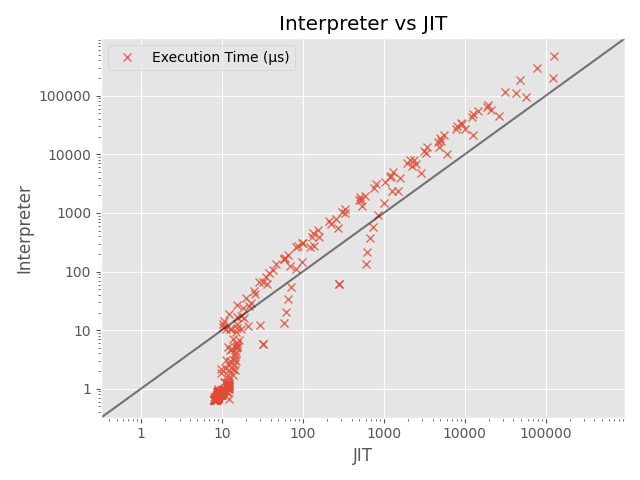
\includegraphics[scale=0.75]{output/graphs/scatter/JIT-vs-Interpreter-time.png}
    \caption{Execution time of all tests for the JIT against the interpreter.}
    \label{figure:time-jit-interpreter}
\end{figure}

\begin{figure}[h]
    \centering
    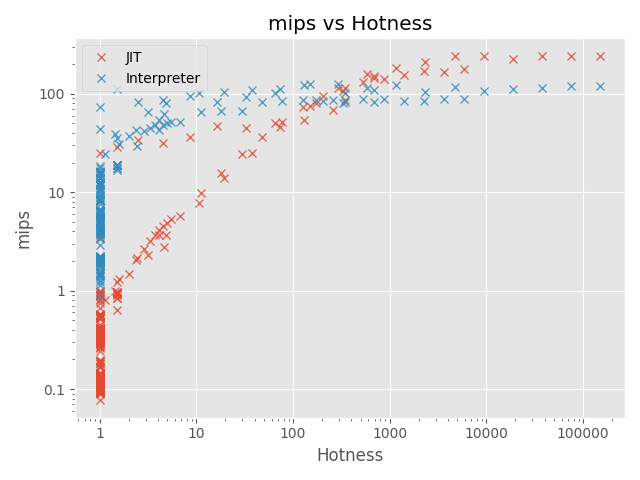
\includegraphics[scale=0.75]{output/graphs/scatter/hotness.png}
    \caption{Performance against hotness for all tests.}
    \label{figure:hotness}
\end{figure}

\subsubsection{Iteration}

\autoref{figure:primal-mips} shows the performance of the \texttt{primal(n)} test suite. It can be seen that as \texttt{n} increases, the performance increases rapidly on both SUTs.

The interpreter has higher initial performance but stabilizes at a lower peak performance and at a lower value of \texttt{n}. This is because the interpreter doesn't speedup much from executing the same blocks repeatedly as there is no caching or reuse involved. It does however still see a large improvement when \texttt{n} is low because at this range the fixed overheads and initialization costs are still relatively high, and hence executing more source instructions amortizes those costs. Furthermore, repeated execution of the same instructions allow the branch predictor to become more accurate and the instruction cache warmer, both contributing to increased performance.

The JIT emulator on the other hand sees a far higher peak performance, but much worse initial performance and takes longer to achieve high performance. This is because, in addition to the higher overhead costs for the JIT emulator, each block of source code also has a high associated compilation costs. As \texttt{n} increases the same blocks are executed many times, amortizing the fixed compilation costs. This allows the JIT emulator to achieve a very high performance due to its far superior execution performance.

\begin{figure}[h]
    \centering
    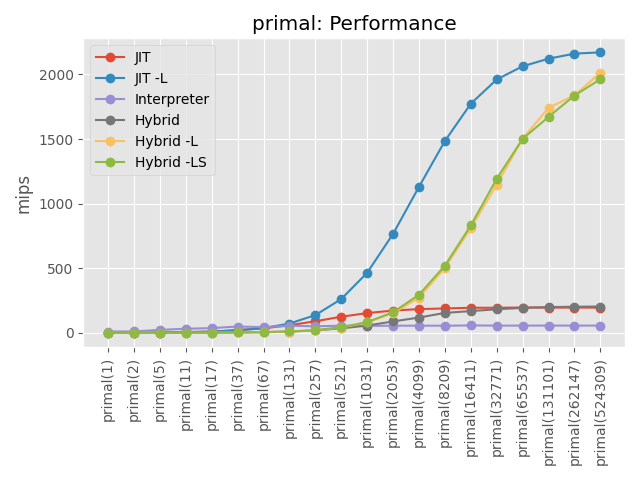
\includegraphics[scale=0.75]{output/graphs/tests/all/primal/mips.png}
    \caption{Performance in mips of the primal test suite.}
    \label{figure:primal-mips}
\end{figure}

\subsubsection{Recursion}

\autoref{figure:fibonacci-mips} shows the performance of the \texttt{fibonacci(n)} test suite. It has a very similar performance characteristic to the \texttt{primal(n)} test suite with some notable differences.

The overall performance for both SUTs is significantly lower. This is due to the memory instructions required for pushing and popping the stack, which have much lower emulation performance compared to arithmetic instructions.

The JIT emulator takes significantly longer to reach peak performance whereas the interpreter does not. This is because the interpreters fixed costs, such as initialization, do not change with the program being executed. The JIT emulator on the other hand has additional costs for every block that needs compiling, and the \texttt{fibonacci(n)} program contains more source blocks. This means there is a larger initial cost which takes longer to amortize.

\begin{figure}[h]
    \centering
    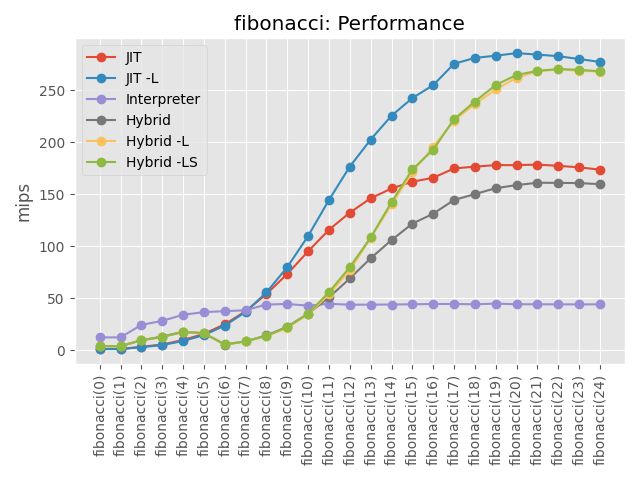
\includegraphics[scale=0.75]{output/graphs/tests/all/fibonacci/mips.png}
    \caption{Performance in mips of the fibonacci test suite.}
    \label{figure:fibonacci-mips}
\end{figure}

\subsubsection{Memory Intensive}

\autoref{figure:memcpyw-mips} shows the performance of the \texttt{memcpyw(n)} test suite. This is the first test suite discussed where performance is not monotonic with regard to \texttt{n} and starts to rapidly fall as \texttt{n} is sufficiently increased.

This is because the more memory copied by the test, the more insertions and accesses are made to the internal hash table powering the memory map. Insertion and access time for the map implementation used becomes slower the more items present in the map \cite{tessil-benchmark}. This linear slowdown is true for all other major C++ unordered map implementations \cite{tessil-benchmark}. This slowdown affects both SUTs as they both internally use the same memory map.

Despite this continuous decrease in performance of the memory map, the overall emulator performance does not monotonically decrease and instead peaks. This is because, for low \texttt{n}, initialization and overhead costs are still being amortized, yielding a performance increase that outweighs the decrease in memory map performance. The JIT emulator has higher overhead costs and thus takes longer to peak. Overall the JIT emulator has higher performance once peaked due to its superior execution performance.

\begin{figure}[h]
    \centering
    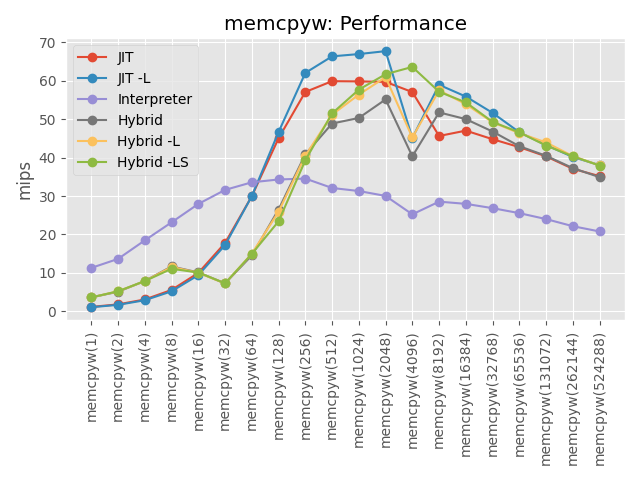
\includegraphics[scale=0.75]{output/graphs/tests/all/memcpyw/mips.png}
    \caption{Performance in mips of the memcpyw test suite.}
    \label{figure:memcpyw-mips}
\end{figure}
